
%\documentclass[calculator,datasheet,solutions,resit]{exam} 
\documentclass[calculator,datasheet,resit]{exam}

% The full list of class options are
% calculator : Allows approved calculator use.
% datasheet : Adds a note that data sheet are attached to the exam.
% handbook : Allows the use of the engineering handbook.
% resit : Adds the resit markings to the paper.
% sample : Adds conspicuous SAMPLE markings to the paper
% solutions : Uses the contents of \solution commands (and \solmarks) to generate a solution file

\usepackage{pdfpages}
\usepackage{lscape,comment}

\coursecode{EG3521}%%
\coursetitle{Engineering Thermodynamics}%

\examtime{00.00--00.00}%
\examdate{00}{06}{2015}%
\examformat{Candidates must attempt \textit{all} questions.}

\newcommand{\frc}{\displaystyle\frac}
\newcommand{\br}[1]{\!\left( #1 \right)}
\newcommand{\abs}[1]{\left| #1 \right|}
\newcommand{\fracd}[2]{\frac{\mathrm{d} #1}{\mathrm{d} #2}}
\newcommand{\fracp}[2]{\frac{\partial #1}{\partial #2}}
\renewcommand{\d}[1]{\mathrm{d} #1 }
\newcommand{\Ma}{\mathrm{M\!a}}



\begin{document}

%%%
%%% QUESTION
%%%
\begin{question}
\begin{enumerate}[(a)]

\item The Rankine cycle is used to convert thermal energy into power. Sketch a Rankine cycle as a pressure enthalpy chart. Describe the cycle.~\marks{8}

\item Given the following information and Mollier chart for the Organic Rankine fluid i-Pentane, estimate the amount of power in kW that could be recovered using a Rankine cycle with an electrical generator coupled to a turbine/expander. The source of heat for the cycle is hot water.
\begin{enumerate}[(i)]
\item Hot water volume  flow = 0.184 m$^{3}$/s
\item Hot water inlet temperature = 95$^{\circ}$C
\item Hot water outlet temperature = 75$^{\circ}$C
\item Hot Water density = 1000 kg/m$^{3}$
\item Hot water specific heat = 4.2 kJ/(kg.$^{\circ}$C)
\end{enumerate}
Assume i-Pentane enters the pump as a saturated liquid at 100 kPa, the pump operates isentropically and the discharge pressure is 350 kPa. Assume the turbine/expander inlet is a saturated vapour. Also, assume the turbine/expander isentropic efficiency is 75$\%$ and the electrical generator efficiency is 90$\%$. State any other assumptions.~\marks{12}
\begin{center}
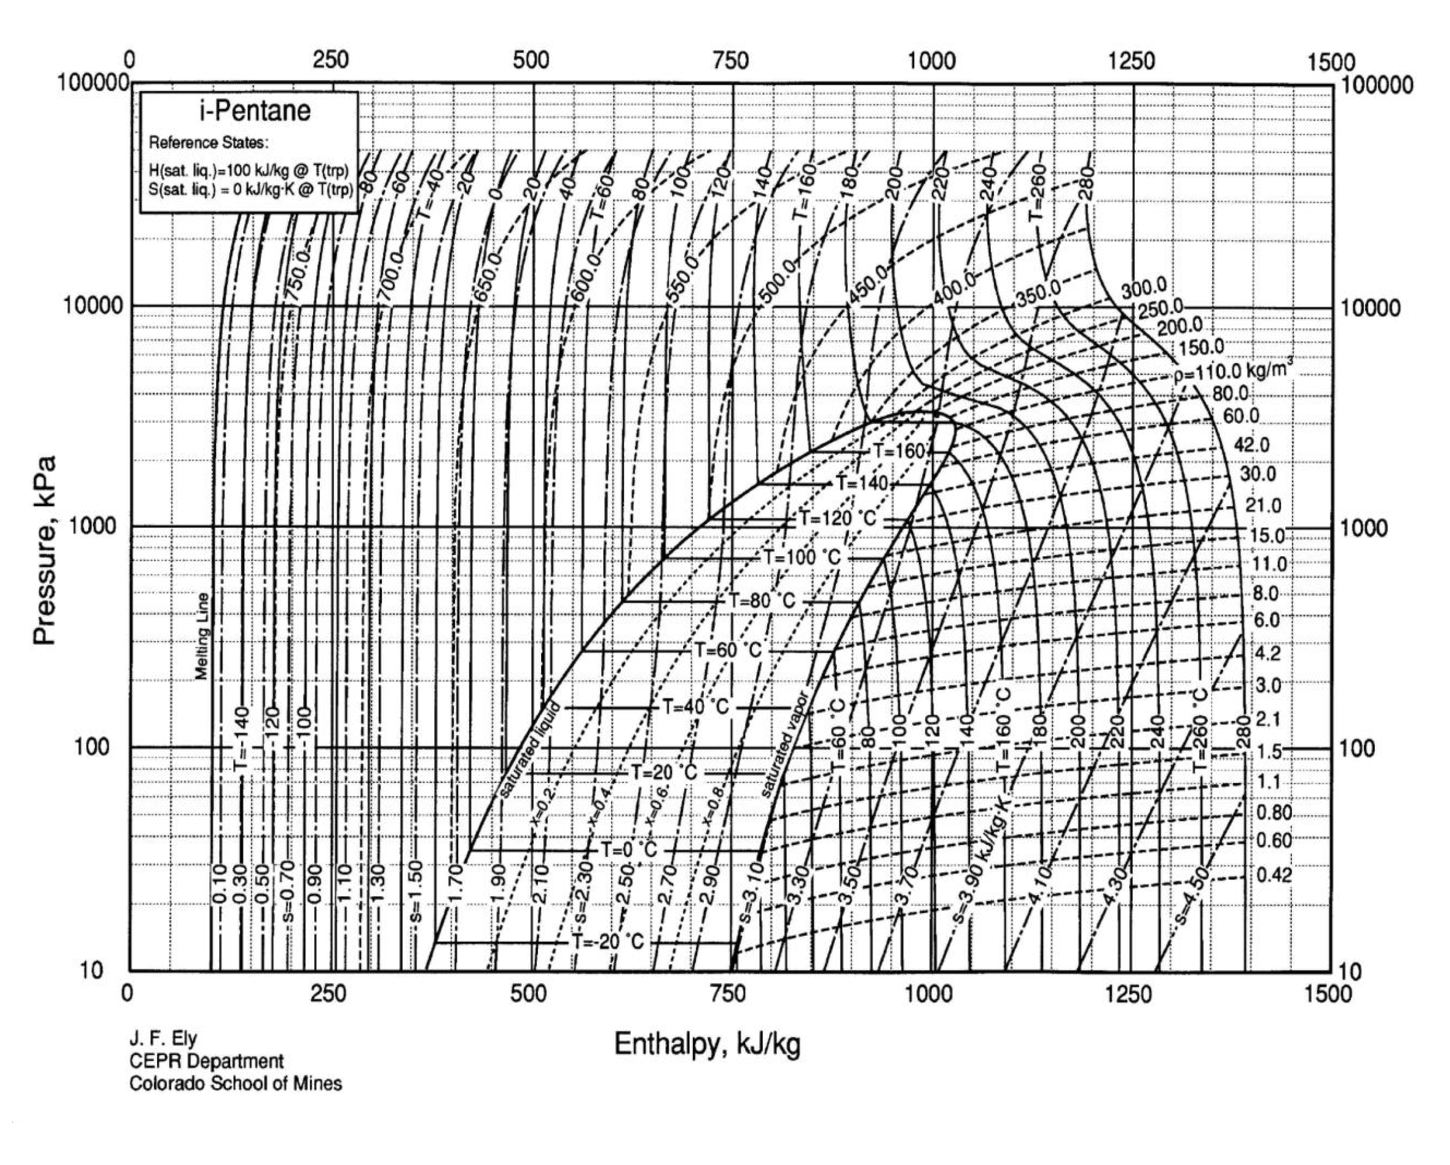
\includegraphics[width=\columnwidth]{./Pics/EG5597_Process_3_June_2014-5.pdf}
\end{center} 


\end{enumerate}
\end{question}

\clearpage

%%% 
%%% QUESTION
%%%
\begin{question}
\begin{enumerate}[(a)]
%
\item An oilfield with a 20 year life has the following energy demand:
\begin{center}
\begin{tabular}{c c |c c |c c |c c}
\hline
{\bf Year} & {\bf Load} & {\bf Year} & {\bf Load} & {\bf Year} & {\bf Load} & {\bf Year} & {\bf Load} \\
           & {\bf MW}   &            &   {\bf MW} &            &  {\bf MW}  &            &   {\bf MW} \\
\hline
1          & 22         & 6          & 24         & 11         & 24         & 16         & 24 \\
2          & 22         & 7          & 24         & 12         & 24         & 17         & 24 \\
3          & 22         & 8          & 26         & 13         & 24         & 18         & 24 \\
4          & 24         & 9          & 28         & 14         & 24         & 19         & 24 \\
5          & 24         & 10         & 28         & 15         & 24         & 20         & 24 \\
\hline
\end{tabular}
\end{center}
The choice of Gas Turbine to provide this power is between Solar Titan and a Solar Mars. Data for these two machines is as follows:
\begin{center}
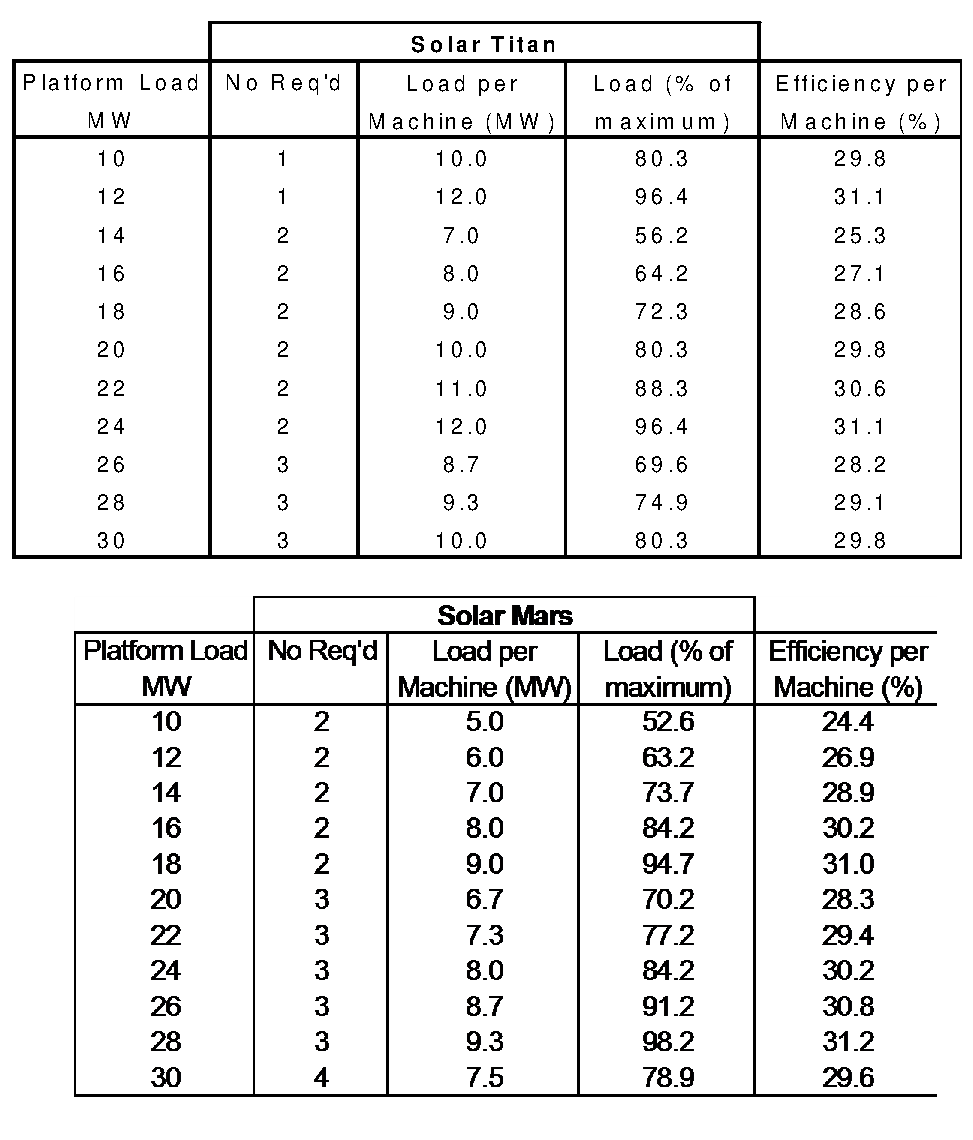
\includegraphics[width=0.8\columnwidth]{./Pics/EG5597_Process_4_June_2014-5.pdf} 
\end{center} 
By conducting an annual review of machine efficiencies and CO$_{2}$ production determine which GT would minimise CO$_{2}$ emissions over the field life.~\marks{12}

\item In order to reduce flaring rates an installation is considering deploying a Flare Gas Recovery System. Sketch and describe the key components of a flare gas recovery system.~\marks{8}


%
\end{enumerate}

\end{question}

\clearpage

%%% 
%%% QUESTION 
%%%
\begin{question}
Answer all of the following questions.

\begin{enumerate}[(a)]
\item Consider the closed-loop block diagram of the process given below, where $K_{p} > 0$, $\tau_{a} > 0$, and $\tau_{b} > 0$. Investigate the stability of the system applying the Routh-Hurwitz stability criterion.~\marks{8}
\begin{center}
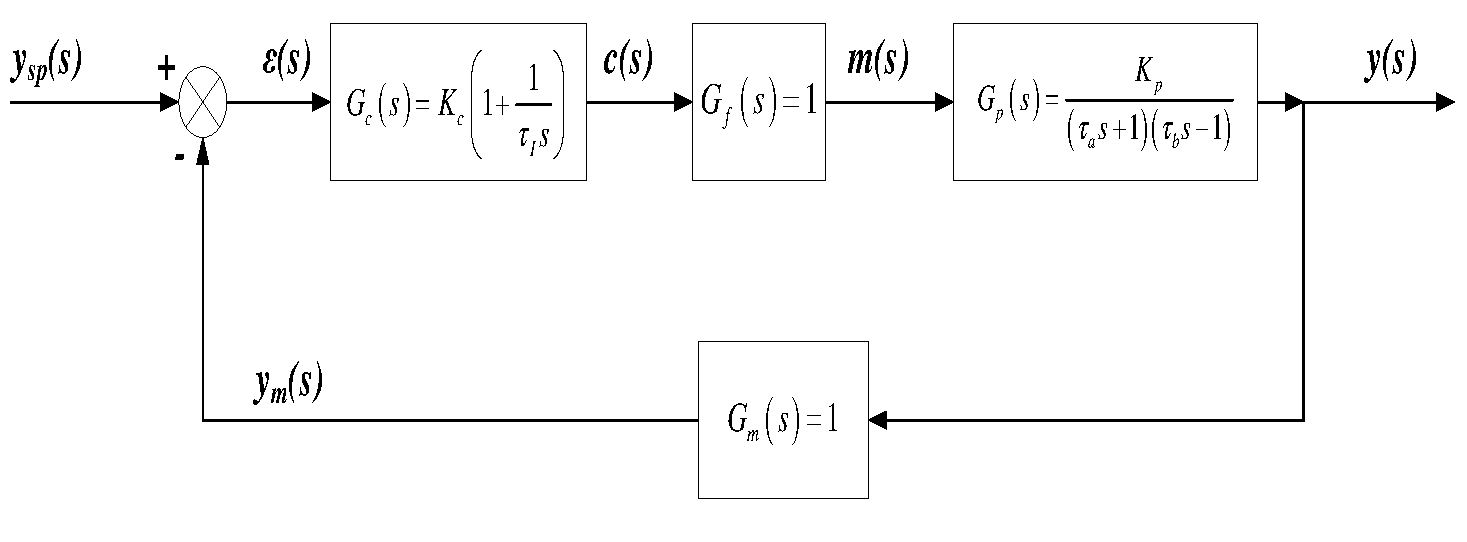
\includegraphics[width=\columnwidth]{./Pics/EG5597_Control_1_June_2014-5.pdf}
\end{center} 

\item Applying the 7 rules for Root-Locus definition, construct the Root-Locus of the closed-loop control system given below. If the Root-Locus crosses the {\it Im}-axis, apply the Routh-Hurwitz stability criterion to find the exact points of intersection. The Root-Locus should be qualitative, but correct on all structural features.~\marks{12}
\begin{center}
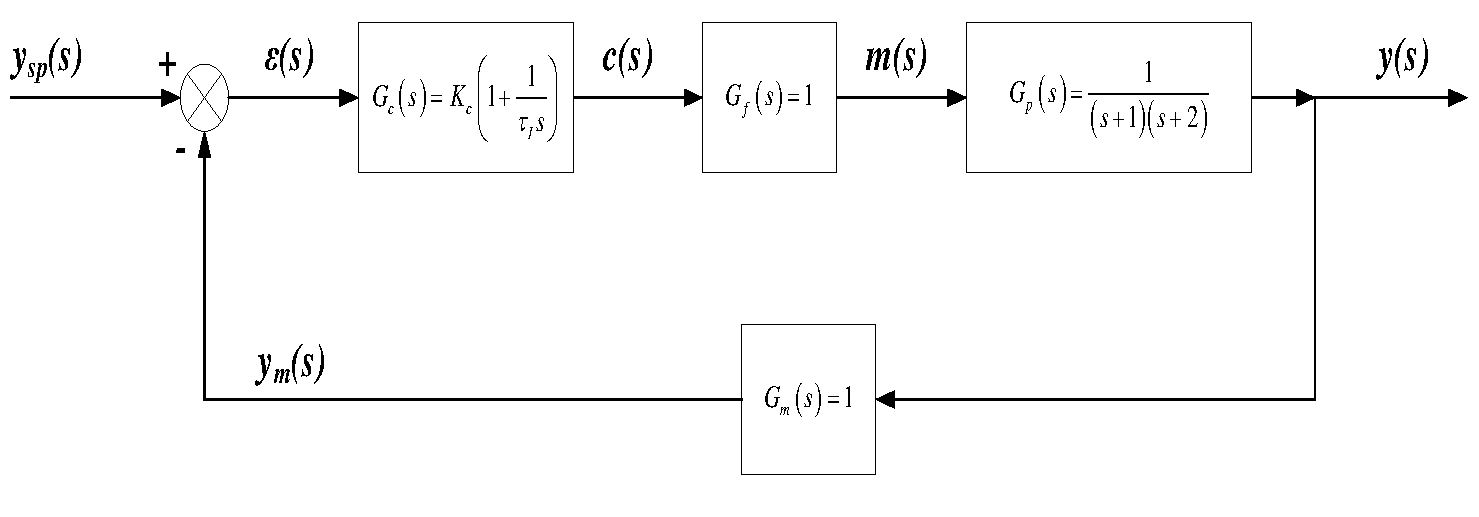
\includegraphics[width=\columnwidth]{./Pics/EG5597_Control_2_June_2014-5.pdf}
\end{center} 
wher $\tau_{I}=0.25$.

\end{enumerate}




\underline{Useful equations}: 
\begin{itemize}
\item Asymptotes angles with positive direction of {\it Re}-axis: 
\begin{displaymath}
\varphi_{i} = \frc{2k + 1}{n -m}\pi,\;\;\;k=0,\cdots,n-m-1
\end{displaymath}

\item Asymptotes centre of gravity:
\begin{displaymath}
\gamma=\frc{\left[\sum\limits_{i=1}^{n}p_{i}-\sum\limits_{j=1}^{m}z_{i}\right]}{(n-m)}
\end{displaymath}

\item Departure/arrival points of branches: 
\begin{displaymath}
\sum\limits_{i=1}^{n}\frc{1}{\left(s_{0}-p_{i}\right)}=\sum\limits_{j=1}^{m}\frc{1}{\left(s_{0}-z_{j}\right)}
\end{displaymath} 
\end{itemize}


\end{question}


\clearpage


%%%%%%%%%%%%%%%%%%%%%%%%%
%%% Question 04       %%%
%%%%%%%%%%%%%%%%%%%%%%%%%
\begin{question} 


\begin{enumerate}[(a)]
\item Gas flows along a pipe of constant cross section $A$\,m$^2$, in the direction of increasing $x$. By considering the rate of change of the mass of gas within a small section of pipe and the gas mass fluxes into and out of this section of pipe, show that
\begin{align*}
 \fracp{\rho}{t} + \fracp{}{x}\left(\rho u\right) = 0.
\end{align*}
Here the gas velocity $u$ and the gas density $\rho$ are functions of $x$ and time $t$. \marks{5} \\
\solution{The total mass contained in a section of pipe of length $\Delta x$ is $\rho A \Delta x$.  \solmarks{1/5}

The rate of change of mass in this section of pipe equals the mass flux entering the pipe $\rho u A$, minus the mass flux leaving the other end of the pipe section
\begin{align*}
 \rho u A + \Delta x \fracp{}{x}\left(\rho u A\right).
\end{align*}
[Obtained via a linearized Taylor expansion.] \solmarks{2/5}

Hence mass conservation implies
\begin{align*}
 \fracp{}{t}\left(\rho A \Delta x\right) = \rho u A - \rho u A - \Delta x \fracp{}{x}\left(\rho u A\right).
\end{align*}
and hence dividing by $A \Delta x$ and rearranging gives the result. \solmarks{2/5}
}

%%%%%%%%%%%
\item Explain what is meant by a steady flow and show that for steady flow in a pipe of constant cross section mass flux is equivalent to
\begin{align*}
 \frac{1}{\rho} \fracd{\rho}{x} + \frac{1}{u} \fracd{u}{x} = 0.
\end{align*} \marks{4}
\solution{The flow is steady if the density, velocity and cross section depend only on $x$ and not time $t$. In this case the result from (a) gives
\begin{align*}
 \fracd{}{x}\left(\rho u\right) = 0.
\end{align*}~\solmarks{2/4}

Therefore via the chain rule
\begin{align*}
 \rho \fracd{u}{x} + u \fracd{\rho}{x} = 0.
\end{align*}
Finally dividing by $\rho u$ gives the required result.\solmarks{2/4}}

%%%%%%%%%%%
\item The beginning of a pipe of constant cross section is located at $x=0$, where the gas velocity into the pipe $u=4$\,m/s. If the gas density profile along the pipe is 
\begin{align*}
 \rho\br{x} = (1 - 0.02x)\,\mbox{kg/m}^3,
\end{align*}
then determine the gas velocity at $x=2$. \marks{7}
\solution{Substituting in the formula from the previous section
\begin{align*}
 \frac{1}{u} \fracd{u}{x} = -\frac{1}{\rho} \fracd{\rho}{x} = -\frac{-0.02}{1 - 0.02x} = \frac{0.02}{1 - 0.02x}.
\end{align*}\solmarks{2/7}

Integrating with respect to $x$
\begin{align*}
 \int_4^u \frac{\d{\tilde{u}}}{\tilde{u}} = \int_0^2 \frac{0.02 \,\d{x}}{1 - 0.02x}.
\end{align*} \solmarks{2/7}

Hence
\begin{align*}
 \left[\log\br{\tilde{u}}\right]_4^u = \left[-\log\br{1 - 0.02x}\right]_0^2,
\end{align*}
\begin{align*}
 \log\br{\frac{u}{4}} = -\log\br{1 - 0.04} + \log\br{1} = \log\br{\frac{1}{0.96}},
\end{align*}\solmarks{1/7}

Exponentiating both sides gives $u = 4/0.96 = 4.1667$\,m/s. \solmarks{2/7}}

%%%%%%%%%%%
\item Gas flows into and out of a steady flow device at a total of three different locations. At the first location gas with density $\rho=1.4$\,kg/m$^3$ flows into the device with velocity $u=4$\,m/s  through a pipe of cross section $A=0.2$\,m$^2$. At the second location gas with density $0.9$\,k/m$^3$ flows out of the device with velocity $u=5$\,m/s through a pipe of cross section $A=0.4$\,m$^2$. At the third location, determine whether gas is flowing into or out of the device. \marks{4}
\solution{The mass flux into the device at the first location is $\rho u A = 1.4\times 4 \times 0.2 = 1.12$\,kg/s. \solmarks{1/4}

The mass flux out of the device at the second location is $\rho u A = 0.9\times 5 \times 0.4 = 1.8$\,kg/s. \solmarks{1/4} 

More gas is flowing out of the device at the second location than is flowing into the device at the first location, and therefore there must be an additional mass flux into the device at the third location. \solmarks{2/4}
}
\end{enumerate}
\end{question}

\clearpage

%%%%%%%%%%%%%%%%%%%%%%%%%
%%% Question 05       %%%
%%%%%%%%%%%%%%%%%%%%%%%%%
\begin{question} 
\begin{enumerate}[(a)]
%%%%%%%%%%%%%%%%%%%%%%%%%%
\item Air in an air-conditioning system is mixed adiabatically with air from outside in a steady process. If the inlets to the mixing chamber are labelled 1 and 2, and the outlet is labelled 3, then state equations that correspond to the mass conservation of dry air, the mass conservation of water vapour and the conservation of energy in this situation. Hence show that
\begin{align*}
 \frac{\dot{m}_{a_1}}{\dot{m}_{a_2}} = \frac{h_3 - h_2}{h_1 - h_3} = \frac{\omega_3 - \omega_2}{\omega_1 - \omega_3},
\end{align*}
where $\dot{m}_a$ is a mass flux of dry air, $h$ is a specific enthalpy and $\omega$ is a specific humidity.\marks{8}
\solution{
In the mixing section
\begin{align*}
\mbox{\textit{Conservation of dry air:}} & & \dot{m}_{a_1} + \dot{m}_{a_2} = \dot{m}_{a_3}, \\
\mbox{\textit{Conservation of water vapour:}} & & \dot{m}_{a_1} \omega_1 + \dot{m}_{a_2} \omega_2 = \dot{m}_{a_3} \omega_3, \\
\mbox{\textit{Conservation of energy:}} & & \dot{m}_{a_1} h_1 + \dot{m}_{a_2} h_2 = \dot{m}_{a_3} h_3.
\end{align*}~\solmarks{3/8}

Using the dry air mass conservation equation to eliminate $\dot{m}_{a_3}$ from the other two expressions, gives
\begin{align*}
 \dot{m}_{a_1} \omega_1 + \dot{m}_{a_2} \omega_2 =& \left(\dot{m}_{a_1} + \dot{m}_{a_2}\right) \omega_3, \\
 \dot{m}_{a_1} h_1 + \dot{m}_{a_2} h_2 =& \left(\dot{m}_{a_1} + \dot{m}_{a_2}\right) h_3.
\end{align*}~\solmarks{2/8}

Collecting all the terms involving $\dot{m}_{a_2}$ on the left-hand side and all the terms involving $\dot{m}_{a_3}$ on the right-hand side gives
\begin{align*}
 \dot{m}_{a_2} \omega_2 - \dot{m}_{a_2} \omega_3 =& \dot{m}_{a_1} \omega_3 - \dot{m}_{a_1} \omega_1, \\
 \dot{m}_{a_2} h_2 - \dot{m}_{a_1} h_3 =& \dot{m}_{a_2} h_3 - \dot{m}_{a_1} h_1.
\end{align*}~\solmarks{1/8}

Rearranging
\begin{align*}
 \dot{m}_{a_2} \left(\omega_3 - \omega_2\right) =& \dot{m}_{a_1} \left(\omega_1 - \omega_3\right), \\
 \dot{m}_{a_2} \left(h_3 - h_2\right) =& \dot{m}_{a_2} \left(h_1 - h_3\right).
\end{align*}~\solmarks{1/8}

Finally
\begin{align*}
 \frac{\dot{m}_{a_1}}{\dot{m}_{a_2}} = \frac{\omega_3 - \omega_2}{\omega_1 - \omega_3}, \quad \mbox{and} \quad \frac{\dot{m}_{a_2}}{\dot{m}_{a_2}} =& \frac{h_3 - h_2}{h_1 - h_3},
\end{align*}
which gives the necessary result.\solmarks{1/8}
}

\item Inlet 1 brings saturated air from the cooling section of the air conditioning system at a temperature of $5^\circ$C. Inlet 2 brings air from outside with a specific humidity of 0.025\,kg water/kg dry air. The resulting mixture is at $20^\circ$C. If liquid water is not produced in the mixing chamber, then determine the minimum temperature of air entering the system through inlet 2. \marks{4}
\solution{Liquid water is not produced in the mixing chamber, so the relative humidity of the mixed gas is equal or less than 100\%. \solmarks{1/4}

On the psychrometric chart the line linking ($T_1=5^\circ$C, $\phi_1=100\%$) and ($T_3=20^\circ$C, $\phi_3=100\%$) intersects the line $\omega_2=0.025\,$kg water/kg dry air when $T_2 = 36^\circ$C. \solmarks{1/4}

Any temperature $T > T_3$ will not produce liquid water in the mixing chamber, so the minimum temperature in inlet 2 is $36^\circ$C. \solmarks{2/4}
}

%%%%%%%%%%%%%%%%%%%%%%%%%%
\item Additionally it is known that the gas mass flux in inlet 2 is twice the gas mass flux in inlet 1.
\begin{enumerate}[(i)]
\item Determine the specific and relative humidity of the mixture. \marks{6}
\solution{From the psychrometric chart the specific humidity of inlet 1 is $\omega_1 = 0.0055$\,kg water/kg dry air.

Rearrange equation part (a) to give
\begin{align*}
 \left(1 + \frac{\dot{m}_{a_1}}{\dot{m}_{a_2}}\right)\omega_3 = \omega_1 + \frac{\dot{m}_{a_1}}{\dot{m}_{a_2}} \omega_2.
\end{align*}\solmarks{2/6}

Therefore
\begin{align*}
 \omega_3 = \frac{0.0055 + \left(0.5\times0.025\right)}{1 + 0.5} = 0.012 \mbox{kg water/kg dry air}.
\end{align*}\solmarks{2/6}

From the psychrometric chart, the relative humidity of the mixture is 82\%. \solmarks{2/6}
}

\item Determine the actual temperature at inlet 2; \marks{2}
\solution{On the psychrometric chart the line linking ($T_1=5^\circ$C, $\phi_1=100\%$) and ($T_3=5^\circ$C, $\omega_3=0.012$\,kg water/kg dry air) intersects the line $\omega_2=0.025\,$kg water/kg dry air when $T_2 = 48.5^\circ$C. Therefore the temperature of the gas in inlet 2 is $48.5^\circ$C. \solmarks{2/2}}
\end{enumerate}
\end{enumerate}
\end{question}


\vfill


\paperend

%\begin{comment}
%\begin{landscape}
%\begin{center}
%\includegraphics[width=1.5\textwidth]{PsychrometricChart}
%\end{center}
{
  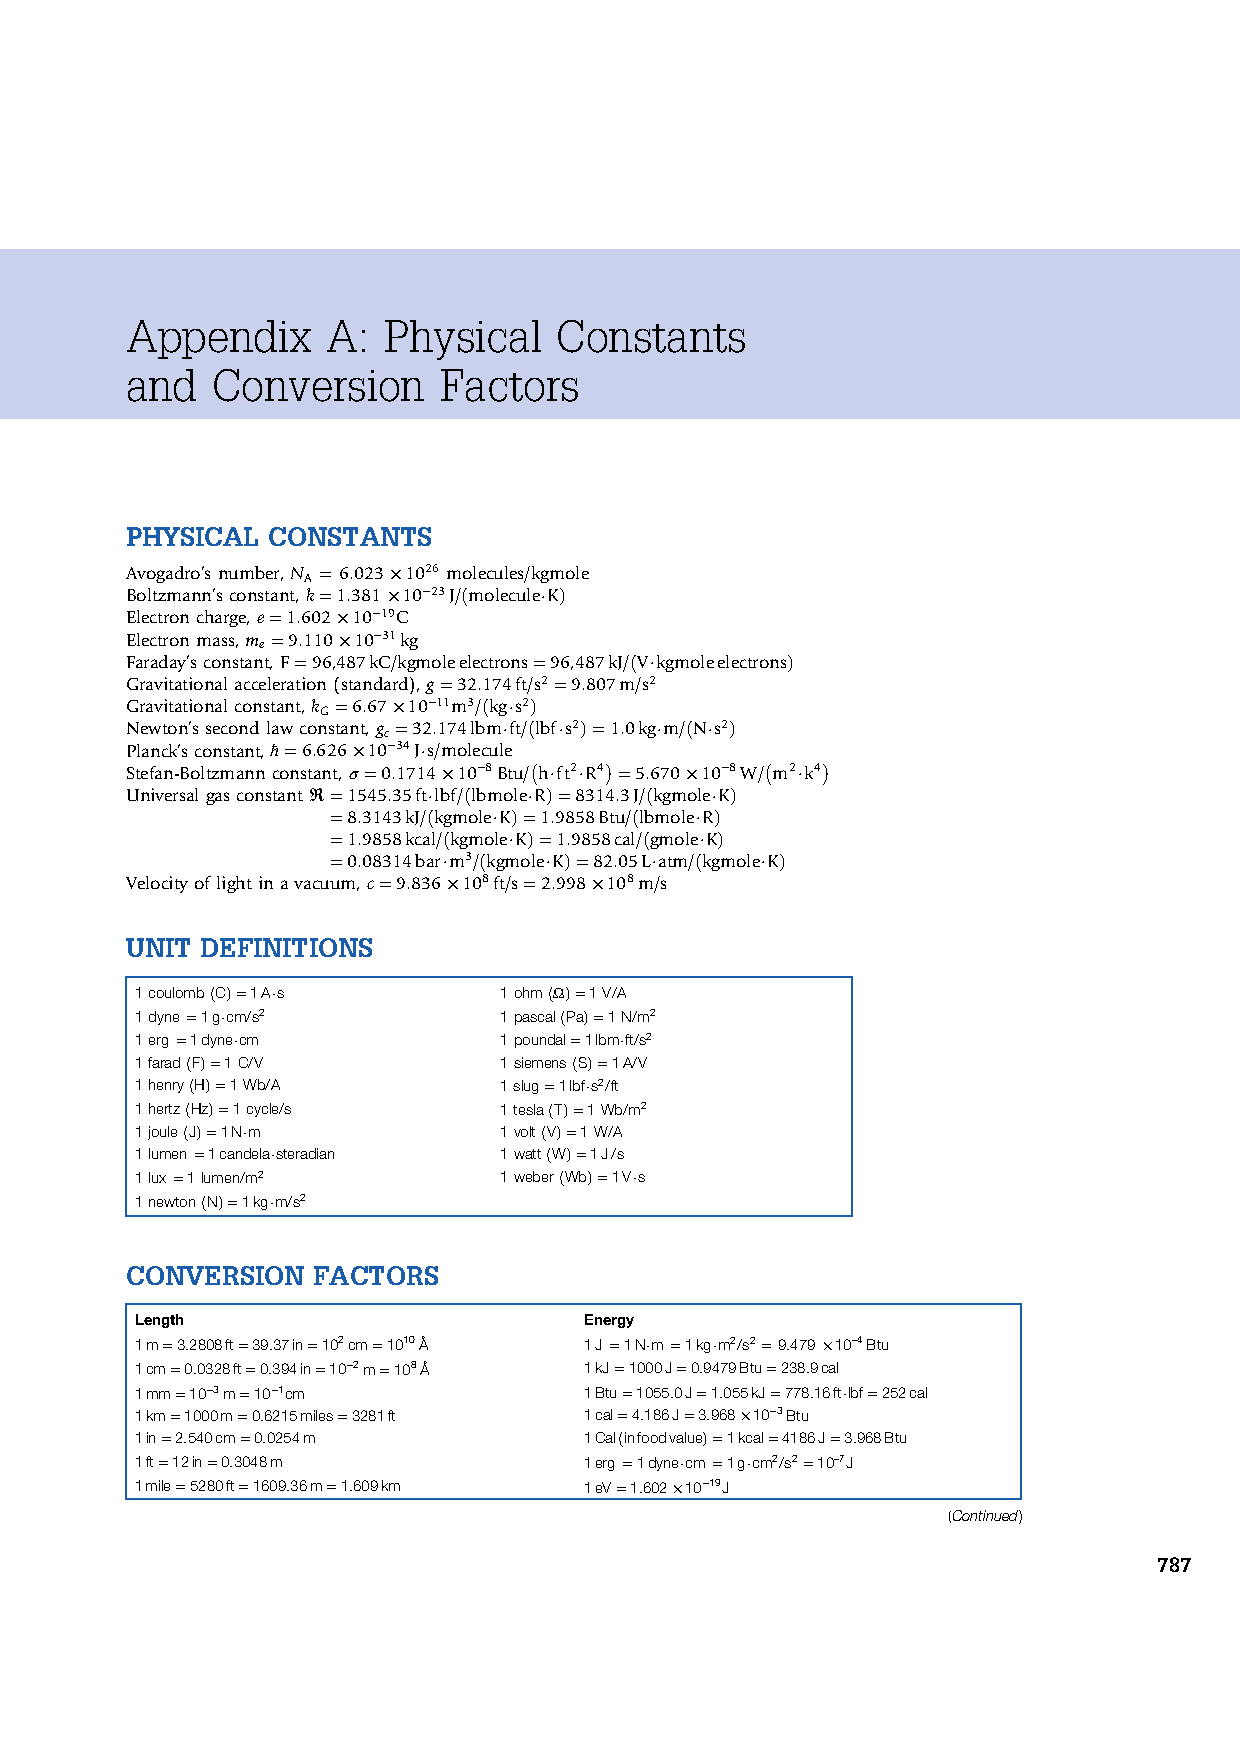
\includepdf[pages=-,fitpaper]{./Pics/UnitConversion}
  \includepdf[pages=-,fitpaper]{./Pics/PsychrometricChart}
  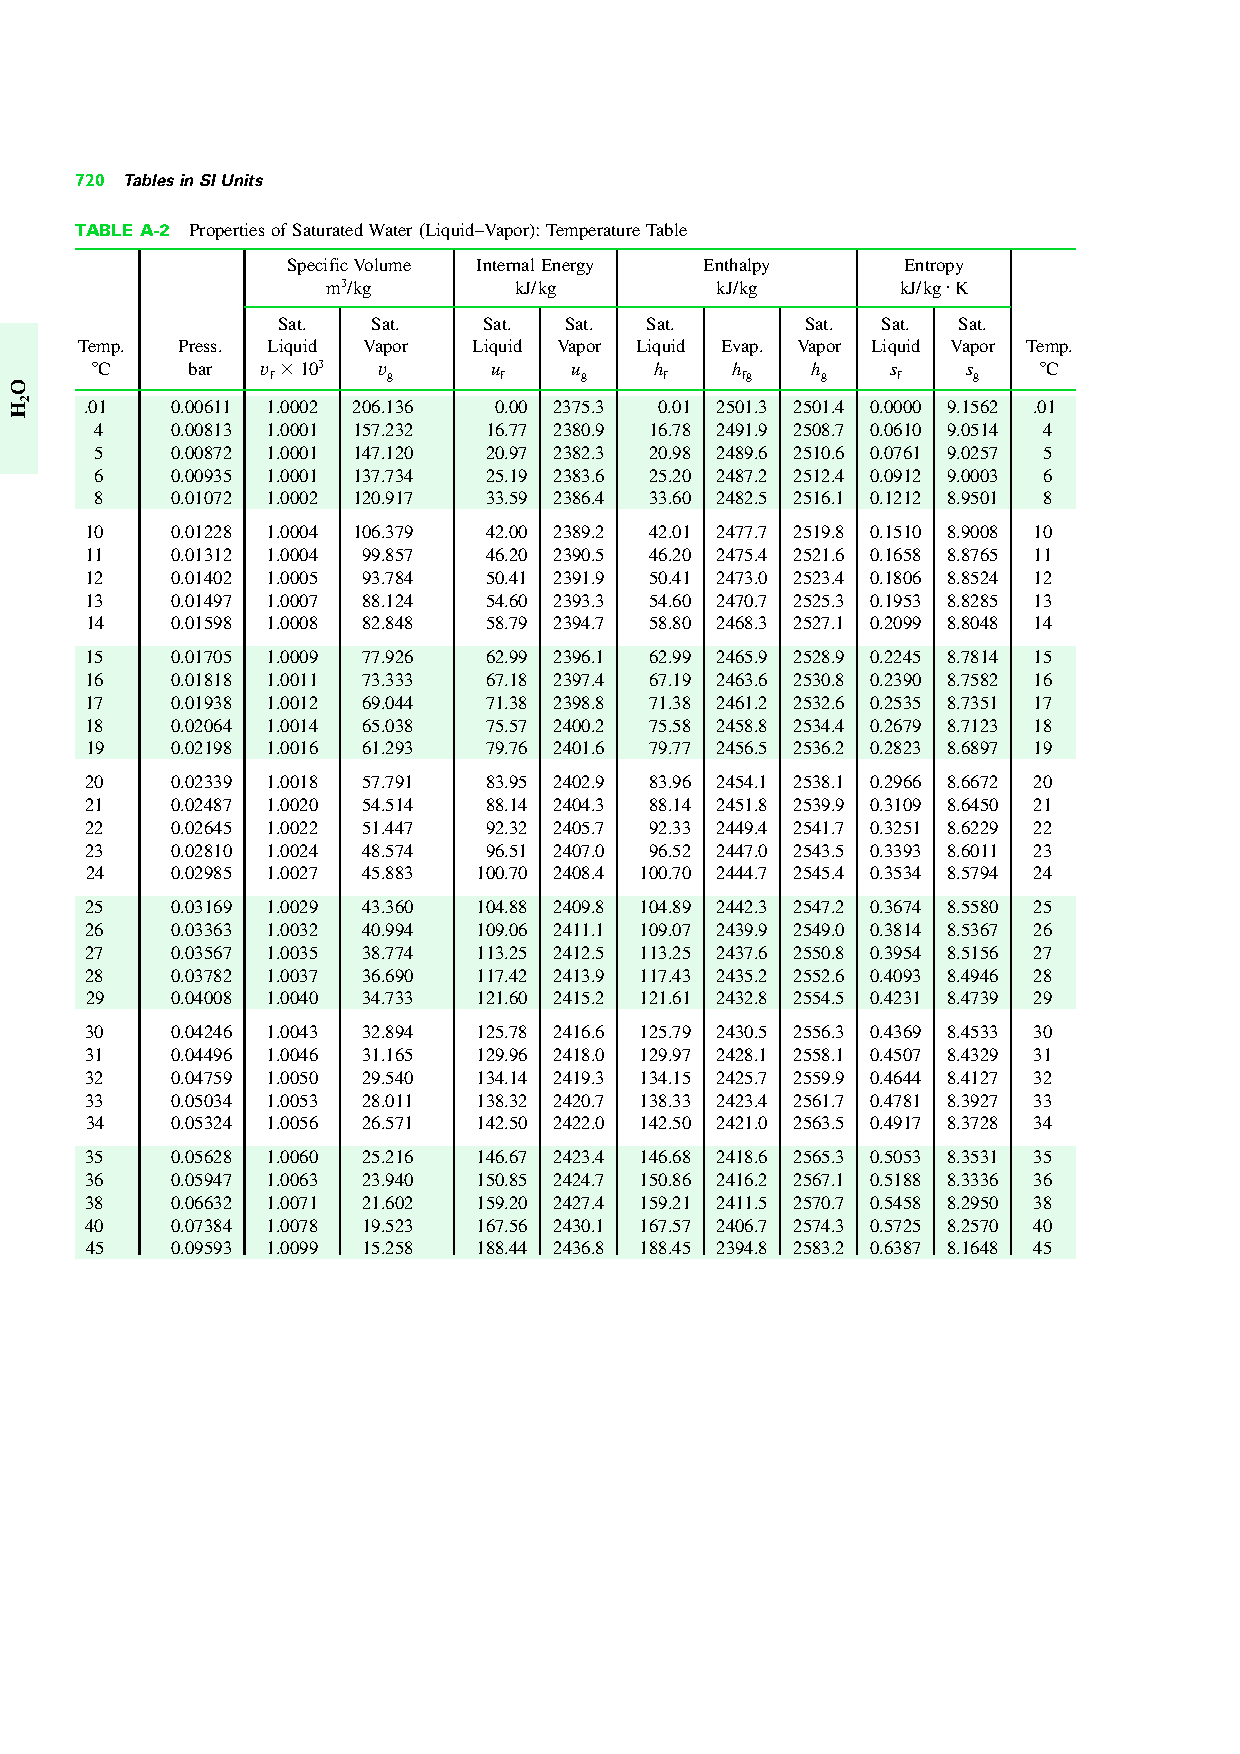
\includepdf[pages=-,fitpaper]{./Pics/H2O-R22_Table}
}
%\end{landscape}
%\end{comment}

\end{document}
